\appendix
\chapter{Appendix}

\section{Statement on the Useage of Gen. AI}
\begin{itemize}
    \item \textbf{Felix Céard-Falkenberg}\newline
Unless stated otherwise, all code, text, and math derivations have been entirely thought and written by me with no external help --- both for gen. AI and wolframalpha anc co.

We used Claude 4.5 Opus for generating the plots for Figure~\ref{fig:mse_naive_better} as the plot is not a core of the assignment, and only aids in understanding our own results. Note that we (heavily) modified the code generated by Claude.

For question 2 of the assignment, we used ChatGPT 5.2 to help us with some of the math of the derivations. The end product is ~90\% my own, indepent work. 
Most of the A.I. being used for question 2 got scrapped as it did not add any value to the report. The most notable scrapped work was finding some result to $\mathbb{E}\left[ \frac{f_1^2}{2f_2} \right]$, but as both are dependent, only very limited results were found by ChatGPT.\!\footnote{This may also be due to my bad prompting.}

% I used ChatGPT to help find literature on the properties of integration, differentiation.

% Furthermore, when researching for denoising algorithms, I used ChatGPT to get a general overview of the available general denoising algorithms. After finding the Bayesian denoising algorithm, I used Claude 4.5 Sonnet to write the code for the Bayesian denoising algorithm (based on existing code for Bayesian denoising implemented for 2D images). As the exact algorithm is not at the core of the assignment or the course, and that the results of both denoising methods are very similar, I believe that this usage is acceptable.


We used Claude 4.5 Opus for generating the plots for Figure~\ref{fig:mse_naive_better} as the plot is not a core of the assignment, and only aids in understanding our own results. Note that we (heavily) modified the code generated by Claude. 

    For Part B, we used ChatGPT to insert some value from lists into latex tables, but we made sure that all values lined up.


    \item \textbf{Yiquan Hu}\newline
    For Part B, we used ChatGPT to generate required code for stepwise selection with the permissions stated in the assignment instructions and also consulted ChatGPT for general suggestions on parameter adjustment. All analysis, results and interpretations were produced by us. We only used ChatGPT lightly refine the academic word of some sentences without adding new content.
    
\end{itemize}

\section{Additional Tables}

\begin{table}[h]
    \centering 
    \caption*{$p_i \sim 0.02 \cdot \mathrm{Beta}(1, 3)$}
    \begin{tabular}{c c|c c c}
        \toprule
        & & \multicolumn{1}{|c|}{${N}=500$} & \multicolumn{1}{c|}{${N}=1000$} & \multicolumn{1}{c}{${N}=5000$} \\
        \midrule
        \multicolumn{2}{c|}{${\hat{\mathbf{N}}}$} & $572.21 \variance{249}$ & $1102.16 \variance{327}$ & $5165.82 \variance{579}$  \\
        \multicolumn{2}{c|}{\textbf{Error} (\%)} & $14.44$ & $10.22$ & $3.32$ \\
        % \hline
        \multicolumn{2}{c|}{${\hat{\mathbf{\sigma}}}_{\hat{N}}$} & $223.18 \variance{168}$ & $288.20 \variance{146}$ & $568.22 \variance{96}$\\
        % \hline
        \multirow{2}{*}{\textbf{C.I.}} & $\alpha = 0.05$ & $[296.06 \variance{80}; 1241.40 \variance{822}]$ & $[688.71 \variance{147}; 1861.17 \variance{749}]$ & $[4189.85 \variance{421}; 6432.61 \variance{798}]$
        \\
        % 
        & $\alpha = 0.01$ & $[248.36 \variance{58}; 1610.48 \variance{1203}]$ & $[602.47 \variance{115}; 2212.82 \variance{975}]$ & $[3932.12 \variance{381}; 6903.90 \variance{882}]$ \\
        \midrule
        \multirow{2}{*}{\textbf{Coverage} (\%)} & $\alpha = 0.05$ & $94.60 \variance{22}$ & $94.00 \variance{23}$ & $94.60 \variance{22}$ \\
        & $\alpha = 0.01$ & $98.90 \variance{10}$ & $98.80 \variance{10}$ & $98.90 \variance{10}$ \\
        \multicolumn{2}{c|}{\textbf{Bias} ($\approx$)} & $5\ 214$ & $10\ 436$ & $27\ 495$ \\
        \multicolumn{2}{c|}{\textbf{Variance} ($\approx$)} & $78\ 120$ & $104\ 540$ & $332\ 210$ \\
        \multicolumn{2}{c|}{\textbf{MSE} ($\approx$)} & $83\ 334$ & $114\ 977$ & $359\ 705$ \\
        \bottomrule
    \end{tabular}
    \caption{Result from $1000$ MC simulations for estimating $\hat{N}$. For each value, we report on the mean (black) and standard deviation (gray). We omit the digits after the decimal point for the standard deviation for brevity.
    The Error (\%) is the absolute difference between the estimated and the true value of $N$, divided by the true value of $N$.}
    \label{tab:problem_2_results_beta_1_3}
\end{table}

\begin{table}[h]
    \centering 
    \caption*{$p_i \sim 0.01 \cdot \mathrm{Beta}(2, 2)$}
    \begin{tabular}{c c|c c c}
        \toprule
        & & \multicolumn{1}{|c|}{${N}=500$} & \multicolumn{1}{c|}{${N}=1000$} & \multicolumn{1}{c}{${N}=5000$} \\
        \midrule
        \multicolumn{2}{c|}{${\hat{\mathbf{N}}}$} & $582.90 \variance{314}$ & $1093.58 \variance{294}$ & $5128.88 \variance{565}$  \\
        \multicolumn{2}{c|}{\textbf{Error} (\%)} & $16.58$ & $9.36$ & $2.58$ \\
        % \hline
        \multicolumn{2}{c|}{${\hat{\mathbf{\sigma}}}_{\hat{N}}$} & $235.15 \variance{275}$ & $281.72 \variance{121}$ & $561.35 \variance{93}$\\
        % \hline
        \multirow{2}{*}{\textbf{C.I.}} & $\alpha = 0.05$ & $[297.63 \variance{84}; 1303.01 \variance{1391}]$ & $[687.38 \variance{139}; 1831.89 \variance{634}]$ & $[4164.29 \variance{411}; 6379.84 \variance{776}]$
        \\
        % 
        & $\alpha = 0.01$ & $[249.11 \variance{59}; 1716.36 \variance{2272}]$ & $[602.16 \variance{110}; 2171.47 \variance{808}]$ & $[3909.42 \variance{373}; 6844.99 \variance{858}]$ \\
        \midrule
        \multirow{2}{*}{\textbf{Coverage} (\%)} & $\alpha = 0.05$ & $95.30 \variance{21}$ & $95.50 \variance{20}$ & $95.40 \variance{20}$ \\
        & $\alpha = 0.01$ & $99.10 \variance{9}$ & $99.10 \variance{9}$ & $98.80 \variance{10}$ \\
        \multicolumn{2}{c|}{\textbf{Bias} ($\approx$)} & $6\ 871$ & $8\ 757$ & $16\ 608$ \\
        \multicolumn{2}{c|}{\textbf{Variance} ($\approx$)} & $131\ 042$ & $94\ 106$ & $323\ 905$ \\
        \multicolumn{2}{c|}{\textbf{MSE} ($\approx$)} & $137\ 913$ & $102\ 864$ & $340\ 514$ \\
        \bottomrule
    \end{tabular}
    \caption{Result from $1000$ MC simulations for estimating $\hat{N}$. For each value, we report on the mean (black) and standard deviation (gray). We omit the digits after the decimal point for the standard deviation for brevity.
    The Error (\%) is the absolute difference between the estimated and the true value of $N$, divided by the true value of $N$.}
    \label{tab:problem_2_results_beta_2_2}
\end{table}

\begin{table}[h]
    \centering 
    \caption*{$p_i \sim U(0, 0.01)$}
    \begin{tabular}{c c|c c c}
        \toprule
        & & \multicolumn{1}{|c|}{${N}=500$} & \multicolumn{1}{c|}{${N}=1000$} & \multicolumn{1}{c}{${N}=5000$} \\
        \midrule
        \multicolumn{2}{c|}{${\hat{\mathbf{N}}}$} & $517.55 \variance{100}$ & $1022.24 \variance{129}$ & $5057.81 \variance{290}$  \\
        \multicolumn{2}{c|}{\textbf{Error} (\%)} & $3.51$ & $2.22$ & $1.16$ \\
        % \hline
        \multicolumn{2}{c|}{${\hat{\mathbf{\sigma}}}_{\hat{N}}$} & $95.08 \variance{31}$ & $130.52 \variance{27}$ & $285.44 \variance{26}$\\
        % \hline
        \multirow{2}{*}{\textbf{C.I.}} & $\alpha = 0.05$ & $[374.85 \variance{57}; 757.81 \variance{181}]$ & $[809.99 \variance{88}; 1328.62 \variance{193}]$ & $[4542.75 \variance{244}; 5664.70 \variance{345}]$
        \\
        % 
        & $\alpha = 0.01$ & $[343.31 \variance{49}; 863.09 \variance{218}]$ & $[757.85 \variance{78}; 1450.54 \variance{219}]$ & $[4397.59 \variance{232}; 5876.88 \variance{364}]$ \\
        \midrule
        \multirow{2}{*}{\textbf{Coverage} (\%)} & $\alpha = 0.05$ & $95.00 \variance{21}$ & $95.20 \variance{21}$ & $94.60 \variance{22}$ \\
        & $\alpha = 0.01$ & $98.80 \variance{10}$ & $99.60 \variance{6}$ & $98.40 \variance{12}$ \\
        \multicolumn{2}{c|}{\textbf{Bias} ($\approx$)} & $307$ & $494$ & $3\ 342$ \\
        \multicolumn{2}{c|}{\textbf{Variance} ($\approx$)} & $10\ 013$ & $17\ 769$ & $82\ 162$ \\
        \multicolumn{2}{c|}{\textbf{MSE} ($\approx$)} & $10\ 321$ & $18\ 263$ & $85\ 504$ \\
        \bottomrule
    \end{tabular}
    \caption{Same configuration as for Table~\ref{tab:problem_2_results_uniform_0_01}, but we run the simulation for twice as long ($T=80$).}
    \label{tab:problem_2_results_extra_long}
\end{table}


\begin{figure}[h]
    \centering
    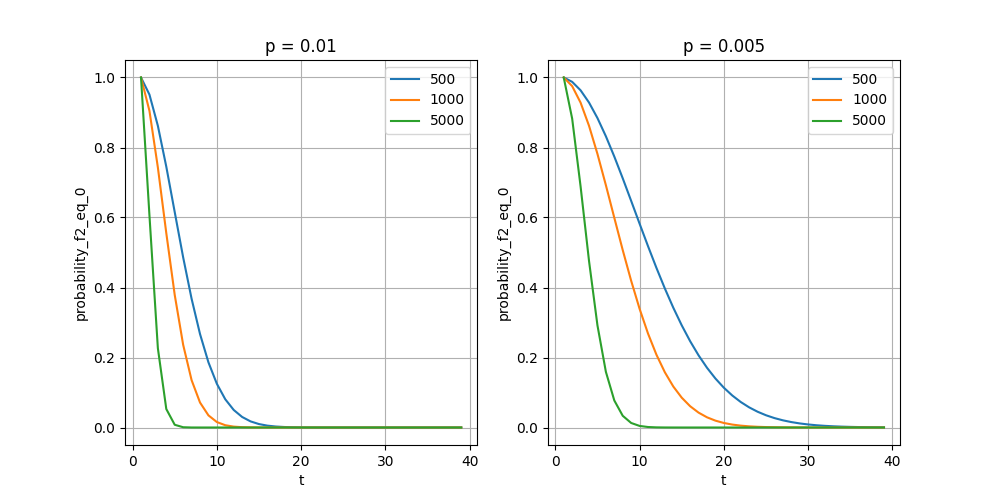
\includegraphics[width=\textwidth]{probability_f2_eq_0.png}
    % 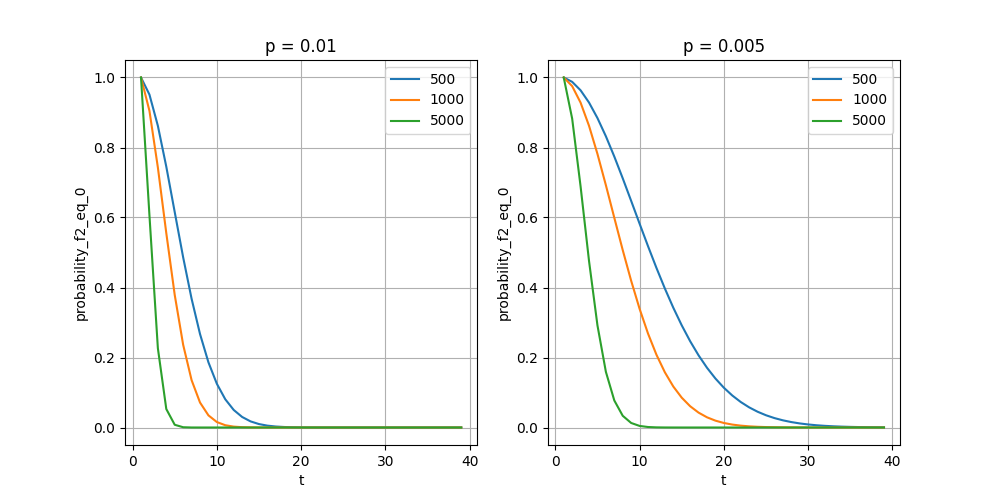
\includegraphics[\linewidth]{probability_f2_eq_0.png}
    \caption{Probability for $f_2 = 0$ over 40 times steps for different population sizes. Note that}
    \label{fig:probability_f2_eq_0_over_time}
\end{figure}

\begin{figure}[h]
    \centering
    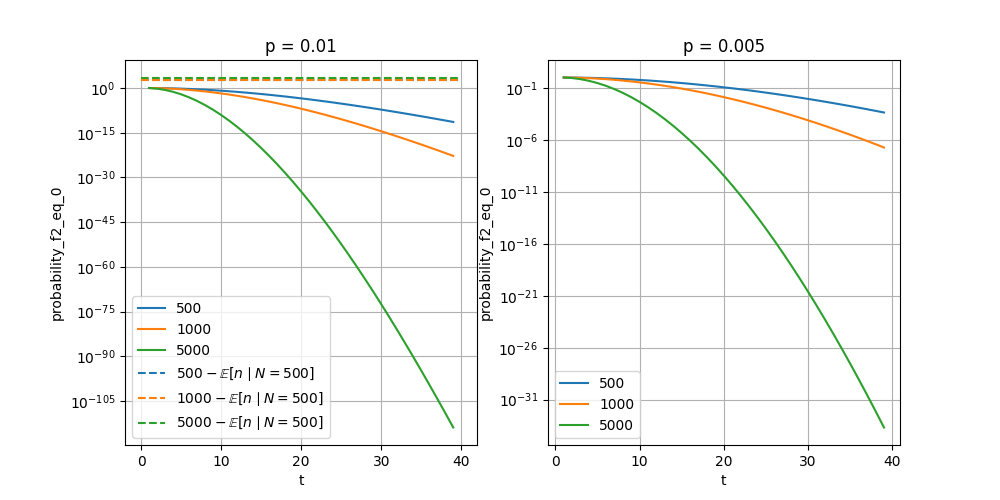
\includegraphics[width=\textwidth]{expectation_f0_f2_eq_0_rescaled.png}
    % 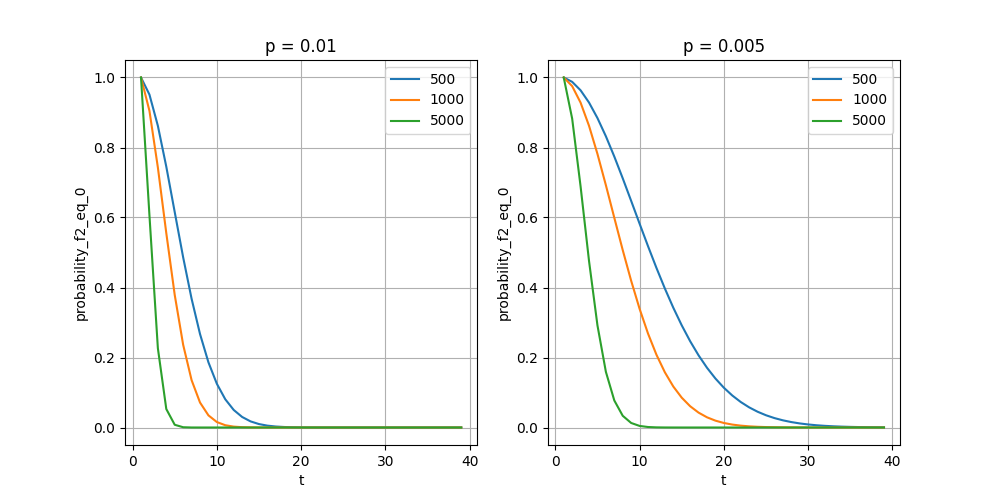
\includegraphics[\linewidth]{probability_f2_eq_0.png}
    \caption{The expected value for $\hat{f_0}$ conditioned on $f_2 = 0$ over 40 times steps for different population sizes. We multiply the expected value by the probability of $f_2 = 0$ at each time step.}
    \label{fig:expectation_f0_f2_eq_0_rescaled}
\end{figure}

\begin{figure}[h]
    \centering
    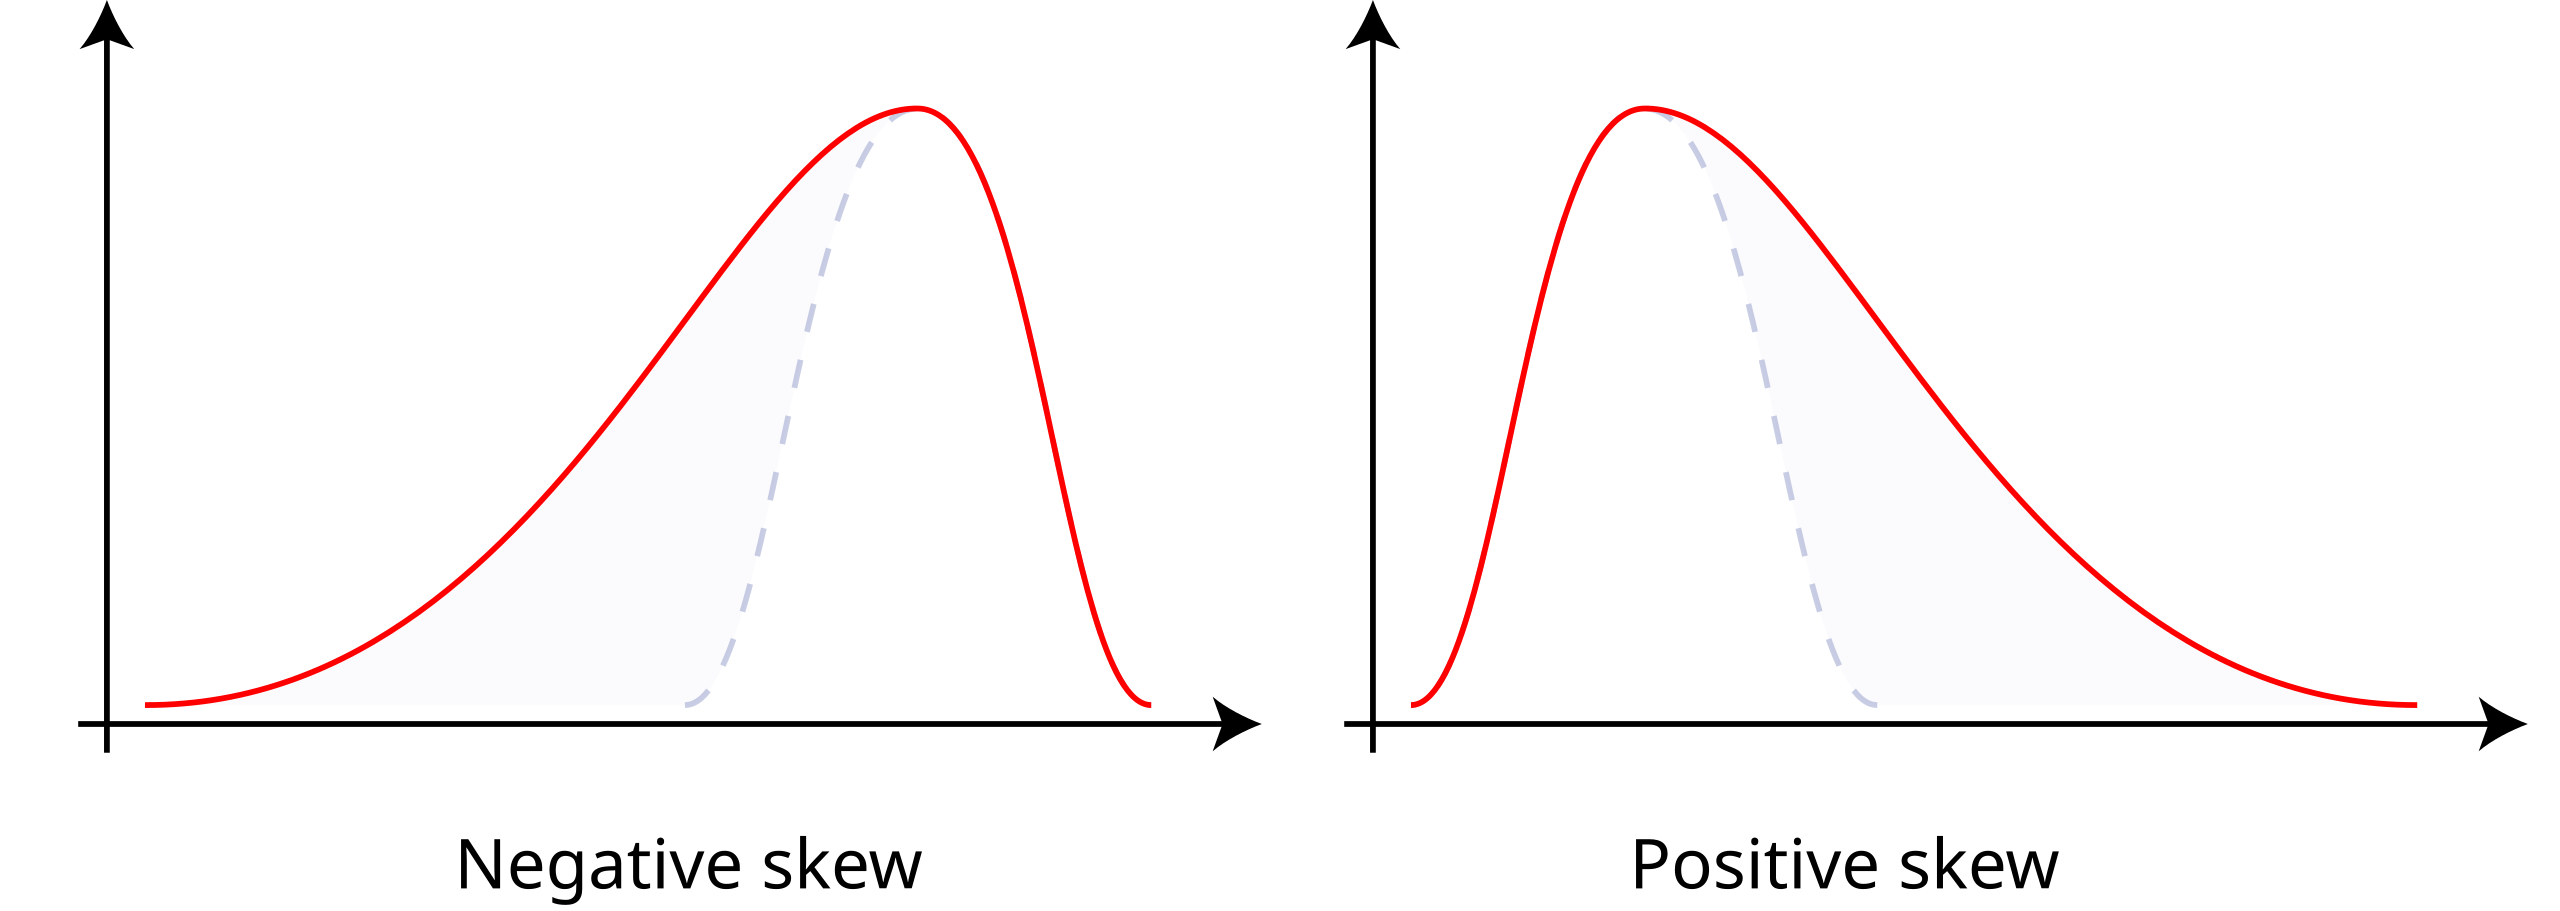
\includegraphics[width=\textwidth]{skewness.png}
    \caption{Interpretation of the skewness of a distribution.}
    \label{fig:interpretation_skewness}
\end{figure}

\pagebreak
\newpage
\subsection{Proof of the dependency of $f_1$ and $f_2$}
\label{sec:proof_dependency_f1_f2}

\begin{tcolorbox}[colframe=red!80!black, colback=red!10, boxrule=1pt, arc=4pt, left=6pt, right=6pt, top=4pt, bottom=4pt]
\textbf{Custom Note:} \\
The idea of this proof is to be credited to ChatGPT.

The current proof is just our own interpretation of the proof generated by ChatGPT, which we have deleted in the mean time.
\end{tcolorbox}

We can model the probability distribution of all $f_k$
jointly as a multinomial distribution.

In statistics, we can define two variables as independent if their covariance is zero.

From the multionomial distribution, we know that the covariance between $f_i$ and $f_j$ is given by 
\begin{equation*}
    \mathrm{Cov}(f_i, f_j) = -N p_i p_j\;.
\end{equation*}

Therefore, we have that 
\begin{align*}
    \mathrm{Cov}(f_1, f_2) &= -N p_1 p_2 \\
    &= -N \cdot \Pr(X_i = 1\mid T=t) \cdot \Pr(X_i = 2 \mid T=t) \\
    &= -N \cdot \mathrm{Binomial}(T, 1, p) \cdot \mathrm{Binomial}(T, 2, p)
\end{align*}
Naturally, we see that the Covariance is not zero, but slightly negative, and therefore the two variables are not independent.

For our four probability distributions, we have the following covariance values:
\begin{table}[h]
    \centering
    \begin{tabular}{c|c c c}
        \toprule
         & \multicolumn{3}{c}{$\mathrm{Cov}(f_1, f_2)$} \\
        \midrule
        $N$ & $500$ & $1000$ & $5000$ \\
        \midrule
        $p=0.01$  & $-7.20$   & $-14.39$  & $-71.95$ \\
        $p=0.005$ & $-1.33$   & $-2.65$   & $-13.26$ \\
        % \bottomrule
    \end{tabular}
    \caption{Covariance for $f_1$ and $f_2$ for $T=40$ and $N \in \{500, 1000, 5000\}$ for different values of $p$.}
    % \label{tab:covariance_f1_f2}
    % \label{tab:expected_value_f0_f2_eq_0}
\end{table}

From the multinomial distribution, we know that the variance of $f_i$ is given by
\begin{equation}
    V(f_i) = N p_i (1-p_i)\;. \label{eq:variance_f_i}
\end{equation}

Therefore, we can use Equation~\ref{eq:variance_f_i} to compute the correlation between $f_1$ and $f_2$ and report it in Table~\ref{tab:correlation_f1_f2}.
\begin{table}[h]
    \centering
    \begin{tabular}{c|c c c}
        \toprule
         & \multicolumn{3}{c}{$\mathrm{Corr}(f_1, f_2)$} \\
        \midrule
        $N$ & $500$ & $1000$ & $5000$ \\
        \midrule
        $p=0.01$  & $-0.1443$   & $-0.1443$  & $-0.1443$ \\
        $p=0.005$ & $-0.0568$   & $-0.0568$  & $-0.0568$ \\
        % \bottomrule
    \end{tabular}
    \caption{Covariance for $f_1$ and $f_2$ for $T=40$ and $N \in \{500, 1000, 5000\}$ for different values of $p$.}
    \label{tab:correlation_f1_f2}
    % \label{tab:expected_value_f0_f2_eq_0}
\end{table}

\qed

\section{Additional Plots and Tables}

\begin{figure}[H]
    \centering
    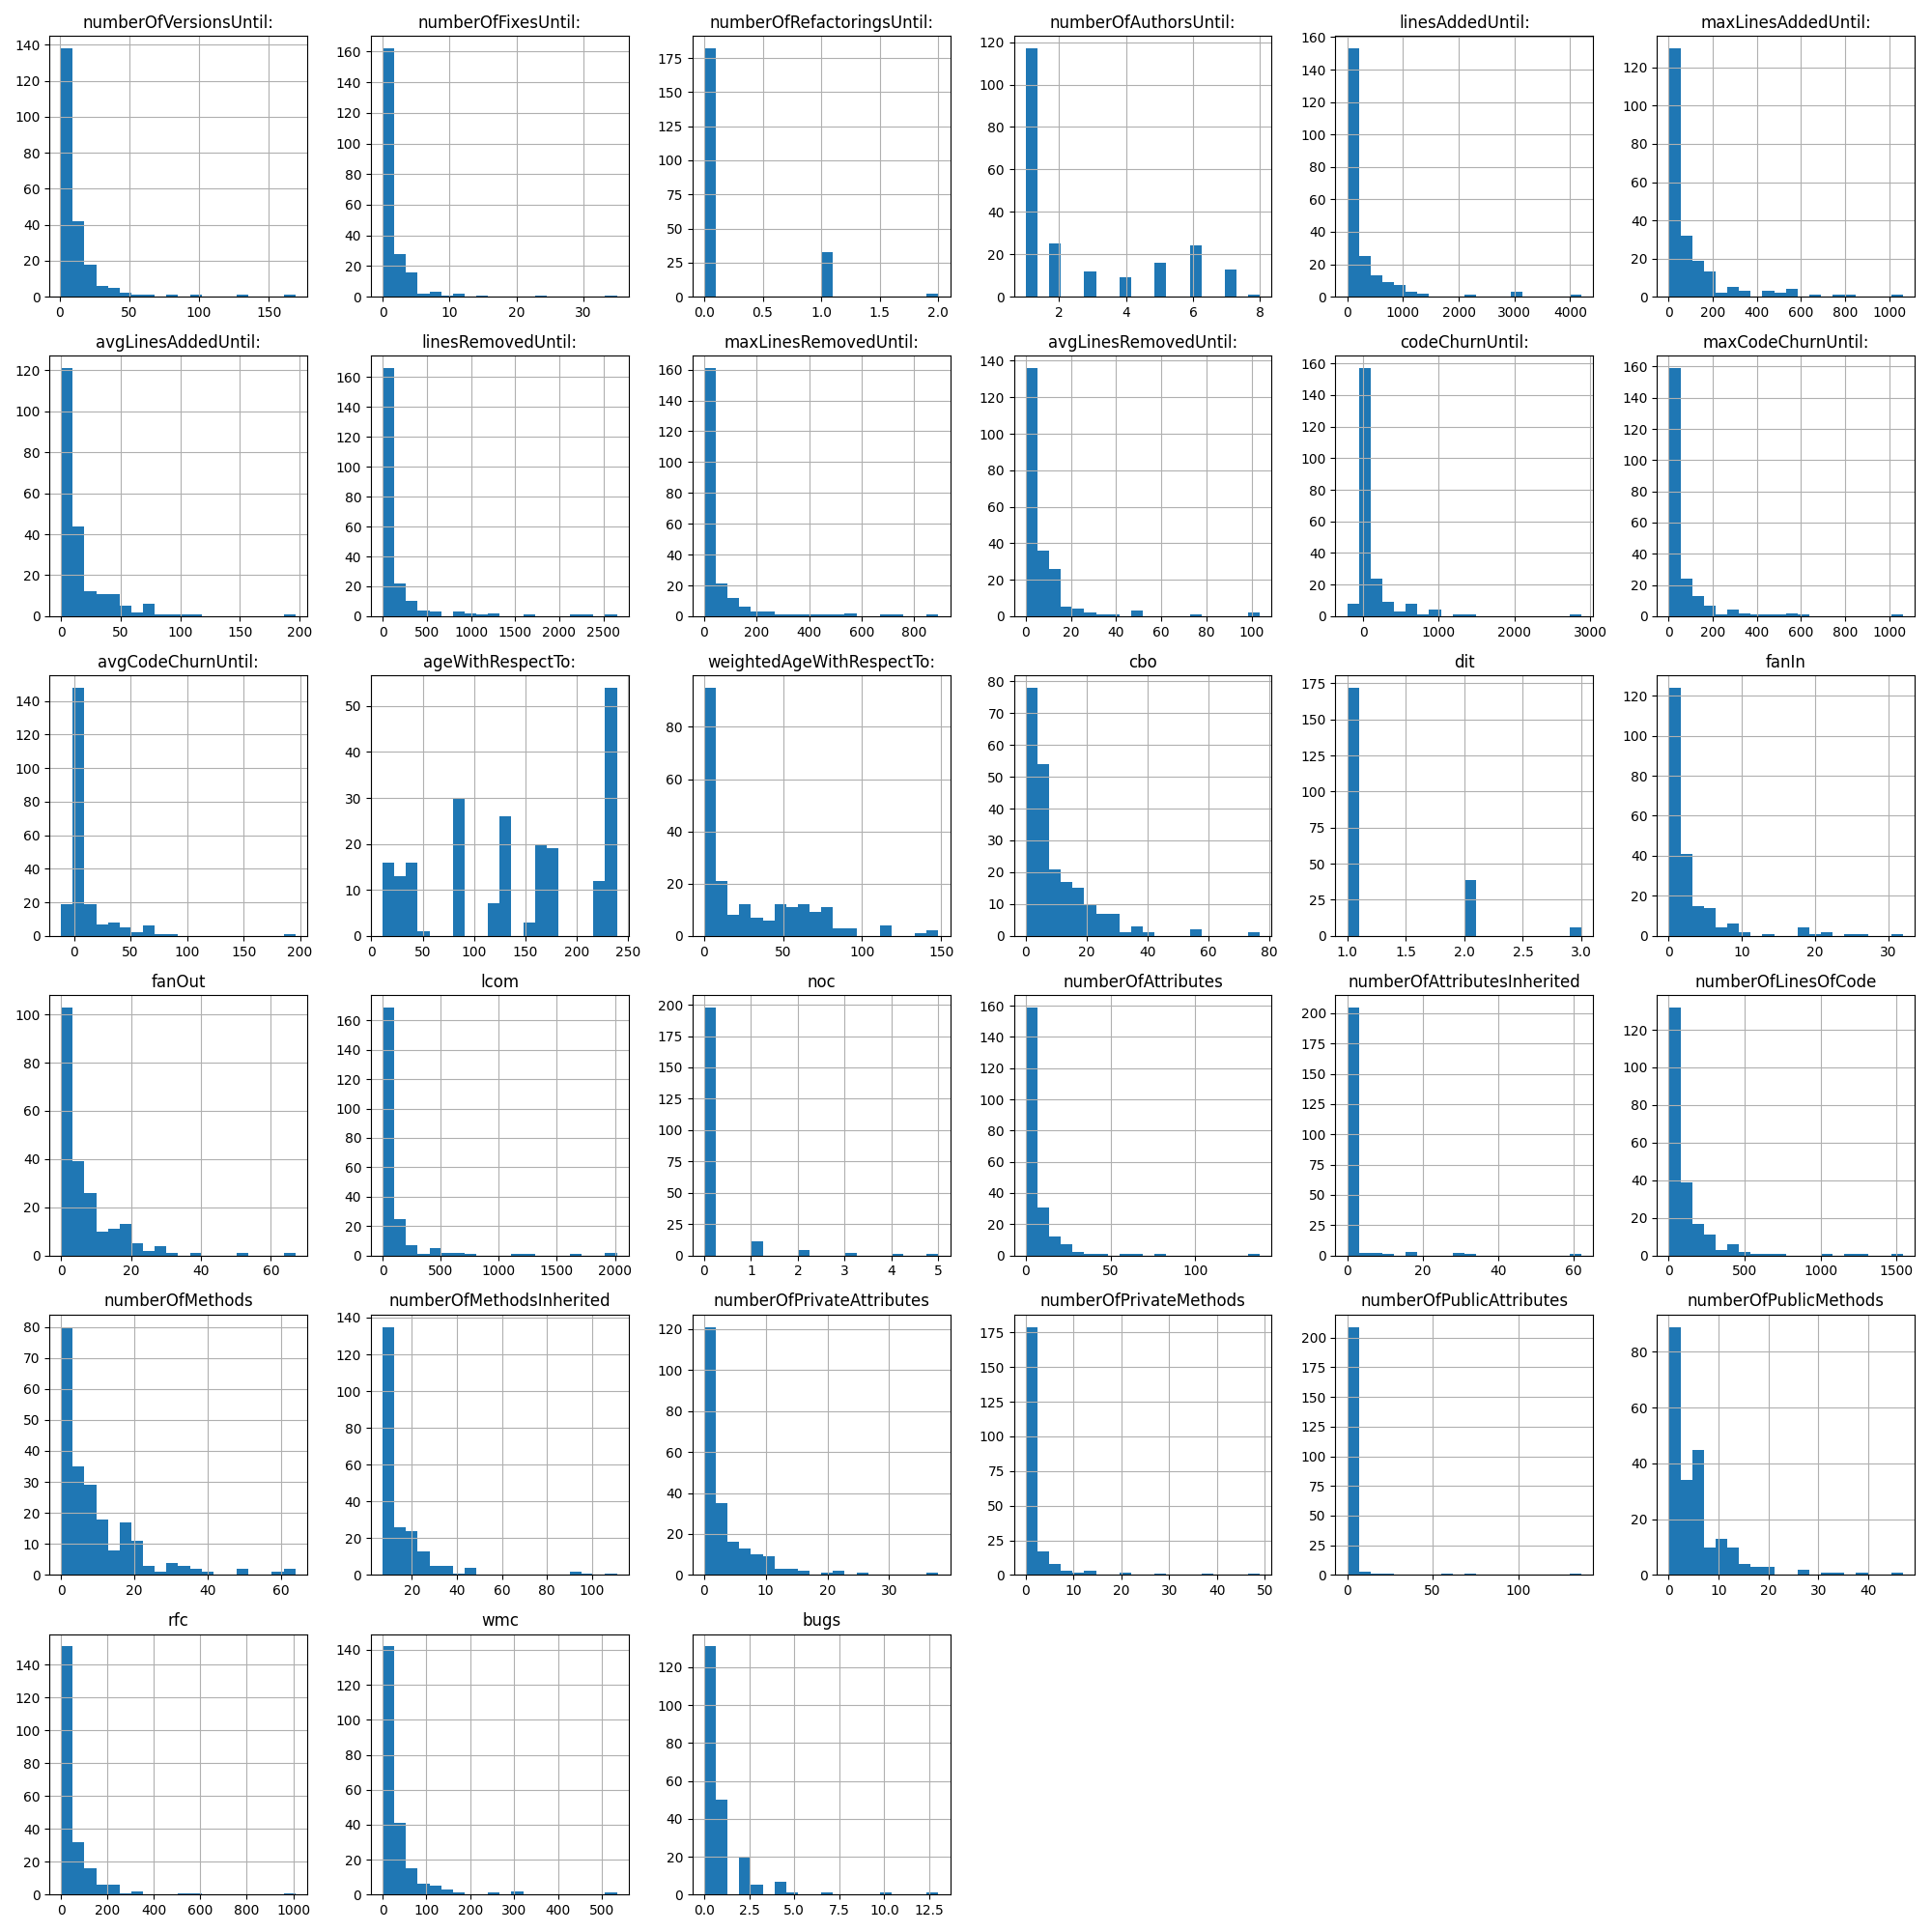
\includegraphics[width=\linewidth]{extra_plots/raw_feature_histograms.png}
    \caption{Histograms of the raw 32 features. No transformation has been applied.}
    \label{fig:feature_histogram_raw}
\end{figure}

\begin{figure}[t]
    \centering
    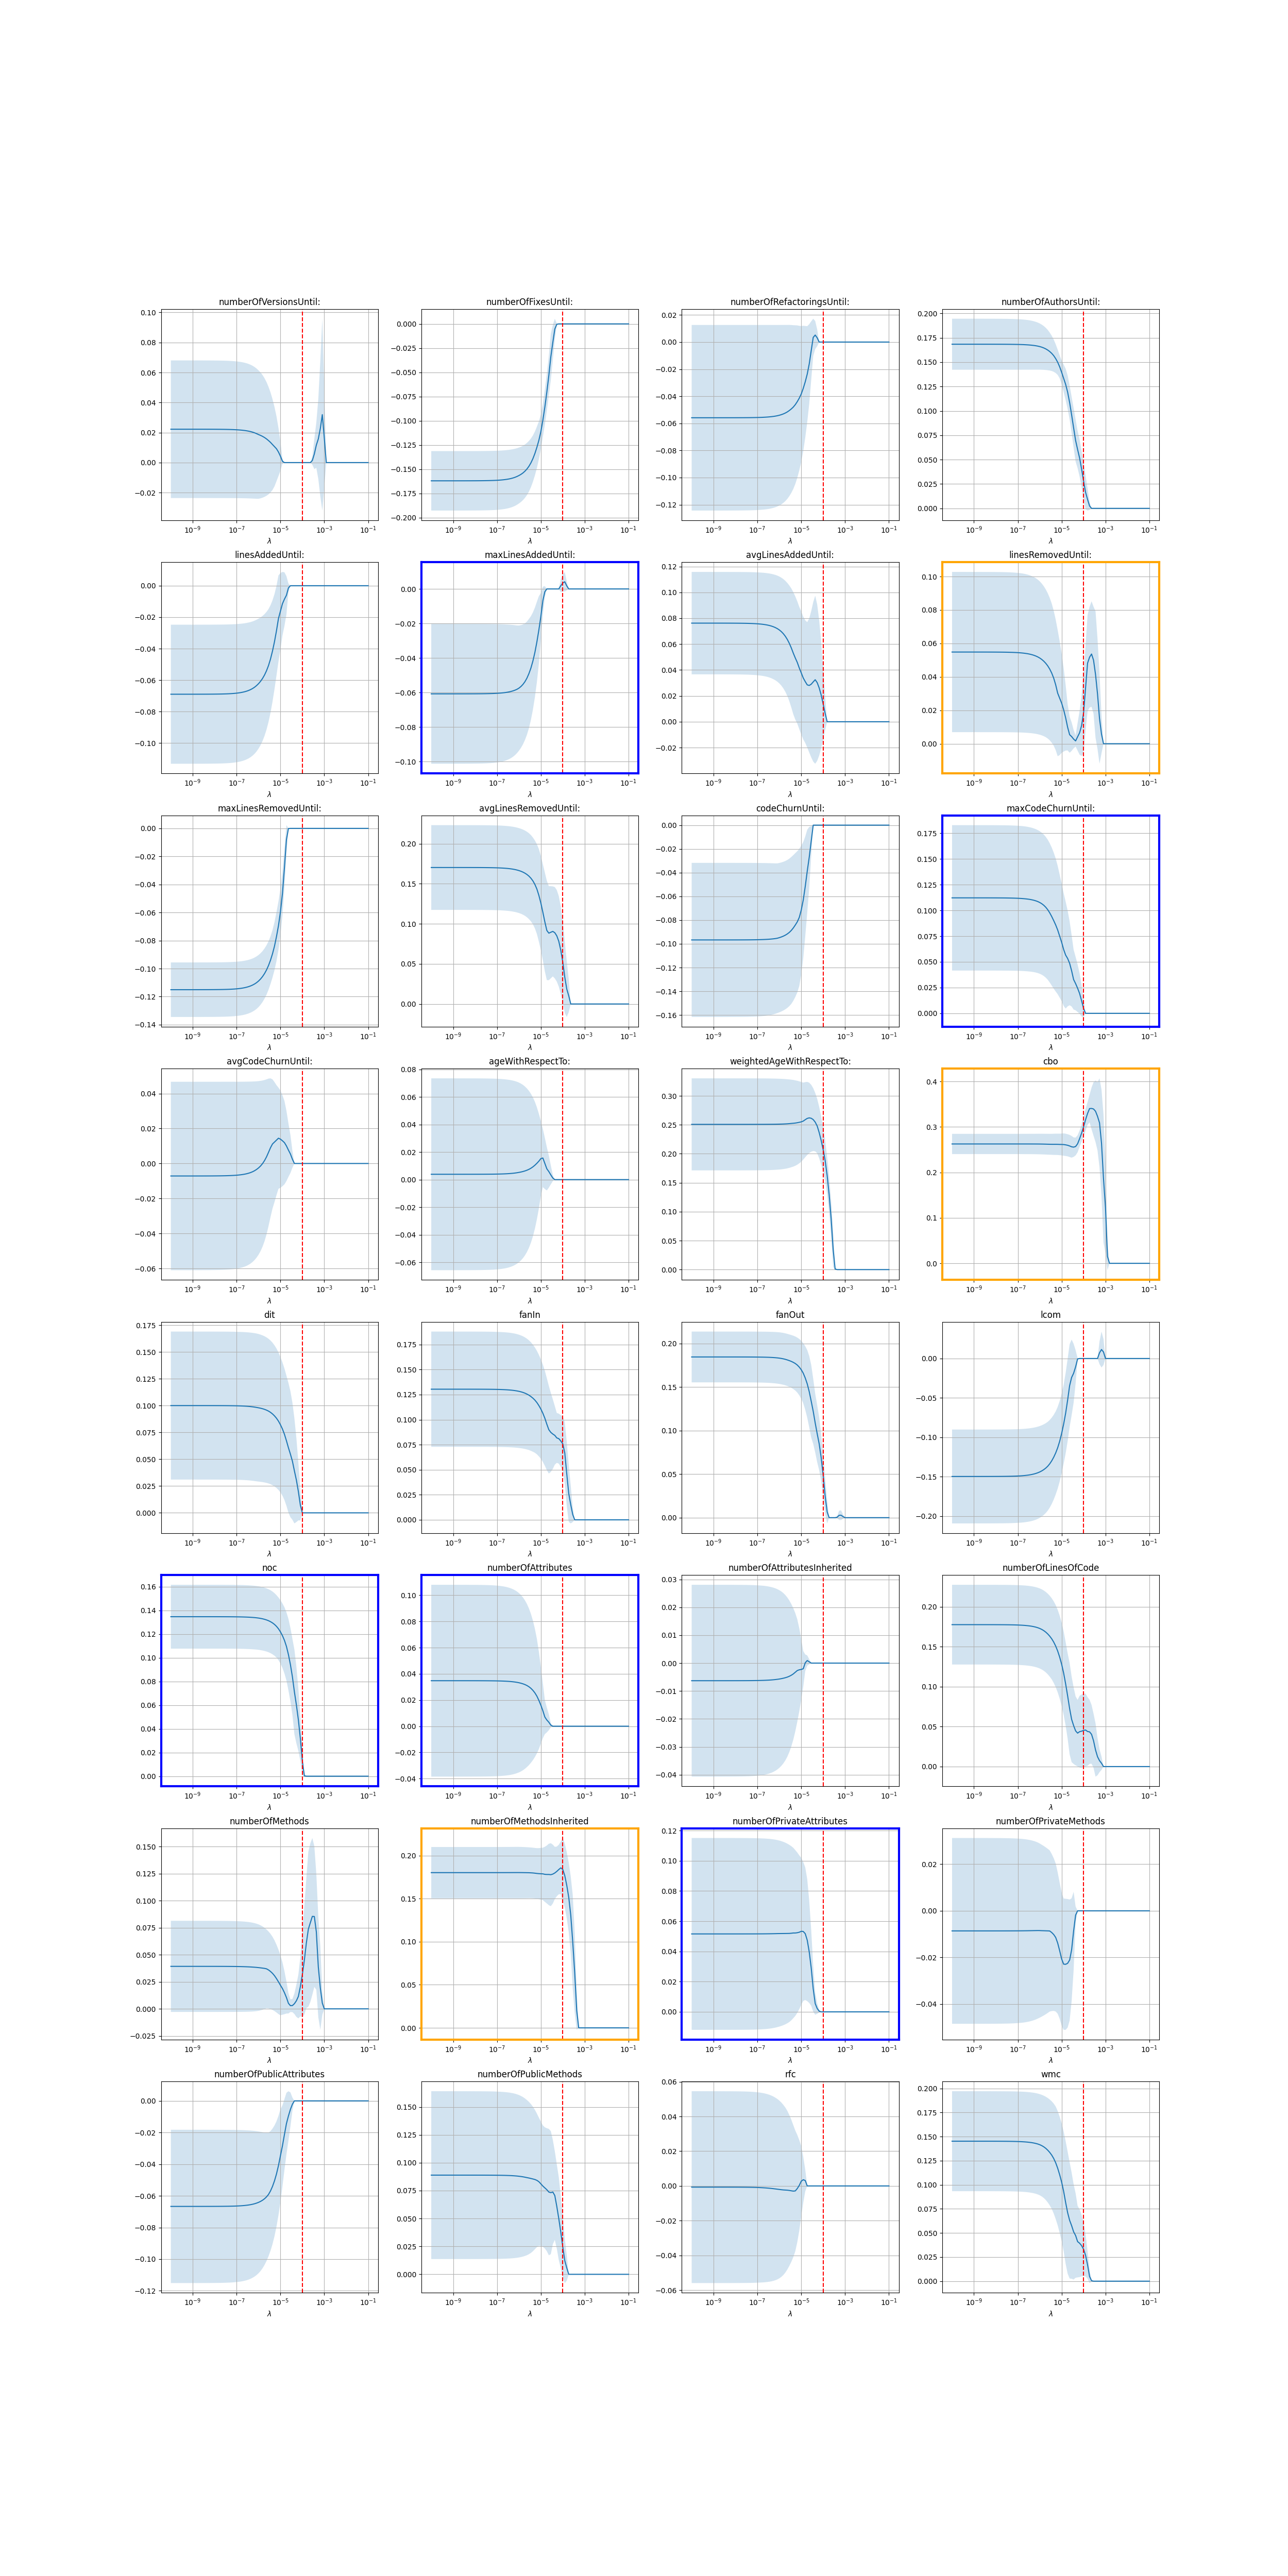
\includegraphics[width=0.5\linewidth]{extra_plots/poisson_regression_lasso_coefficients_no_log_transform.png}
    \caption{The coefficients of the \textbf{Poisson} regression model for all 32 features w.r.t. $\lambda$ when using the \textbf{normalized} data. The plots highlighted in \textbf{blue} are features found by the stepwise search model using AIC. We further highlighted in \textbf{orange} the features found by the stepwise search when using BIC. We advise the reader to view this report digitally to make the most of this plot.}
    \label{fig:coefficients_lambda_normalized}
\end{figure}

\begin{figure}[t]
    \centering
    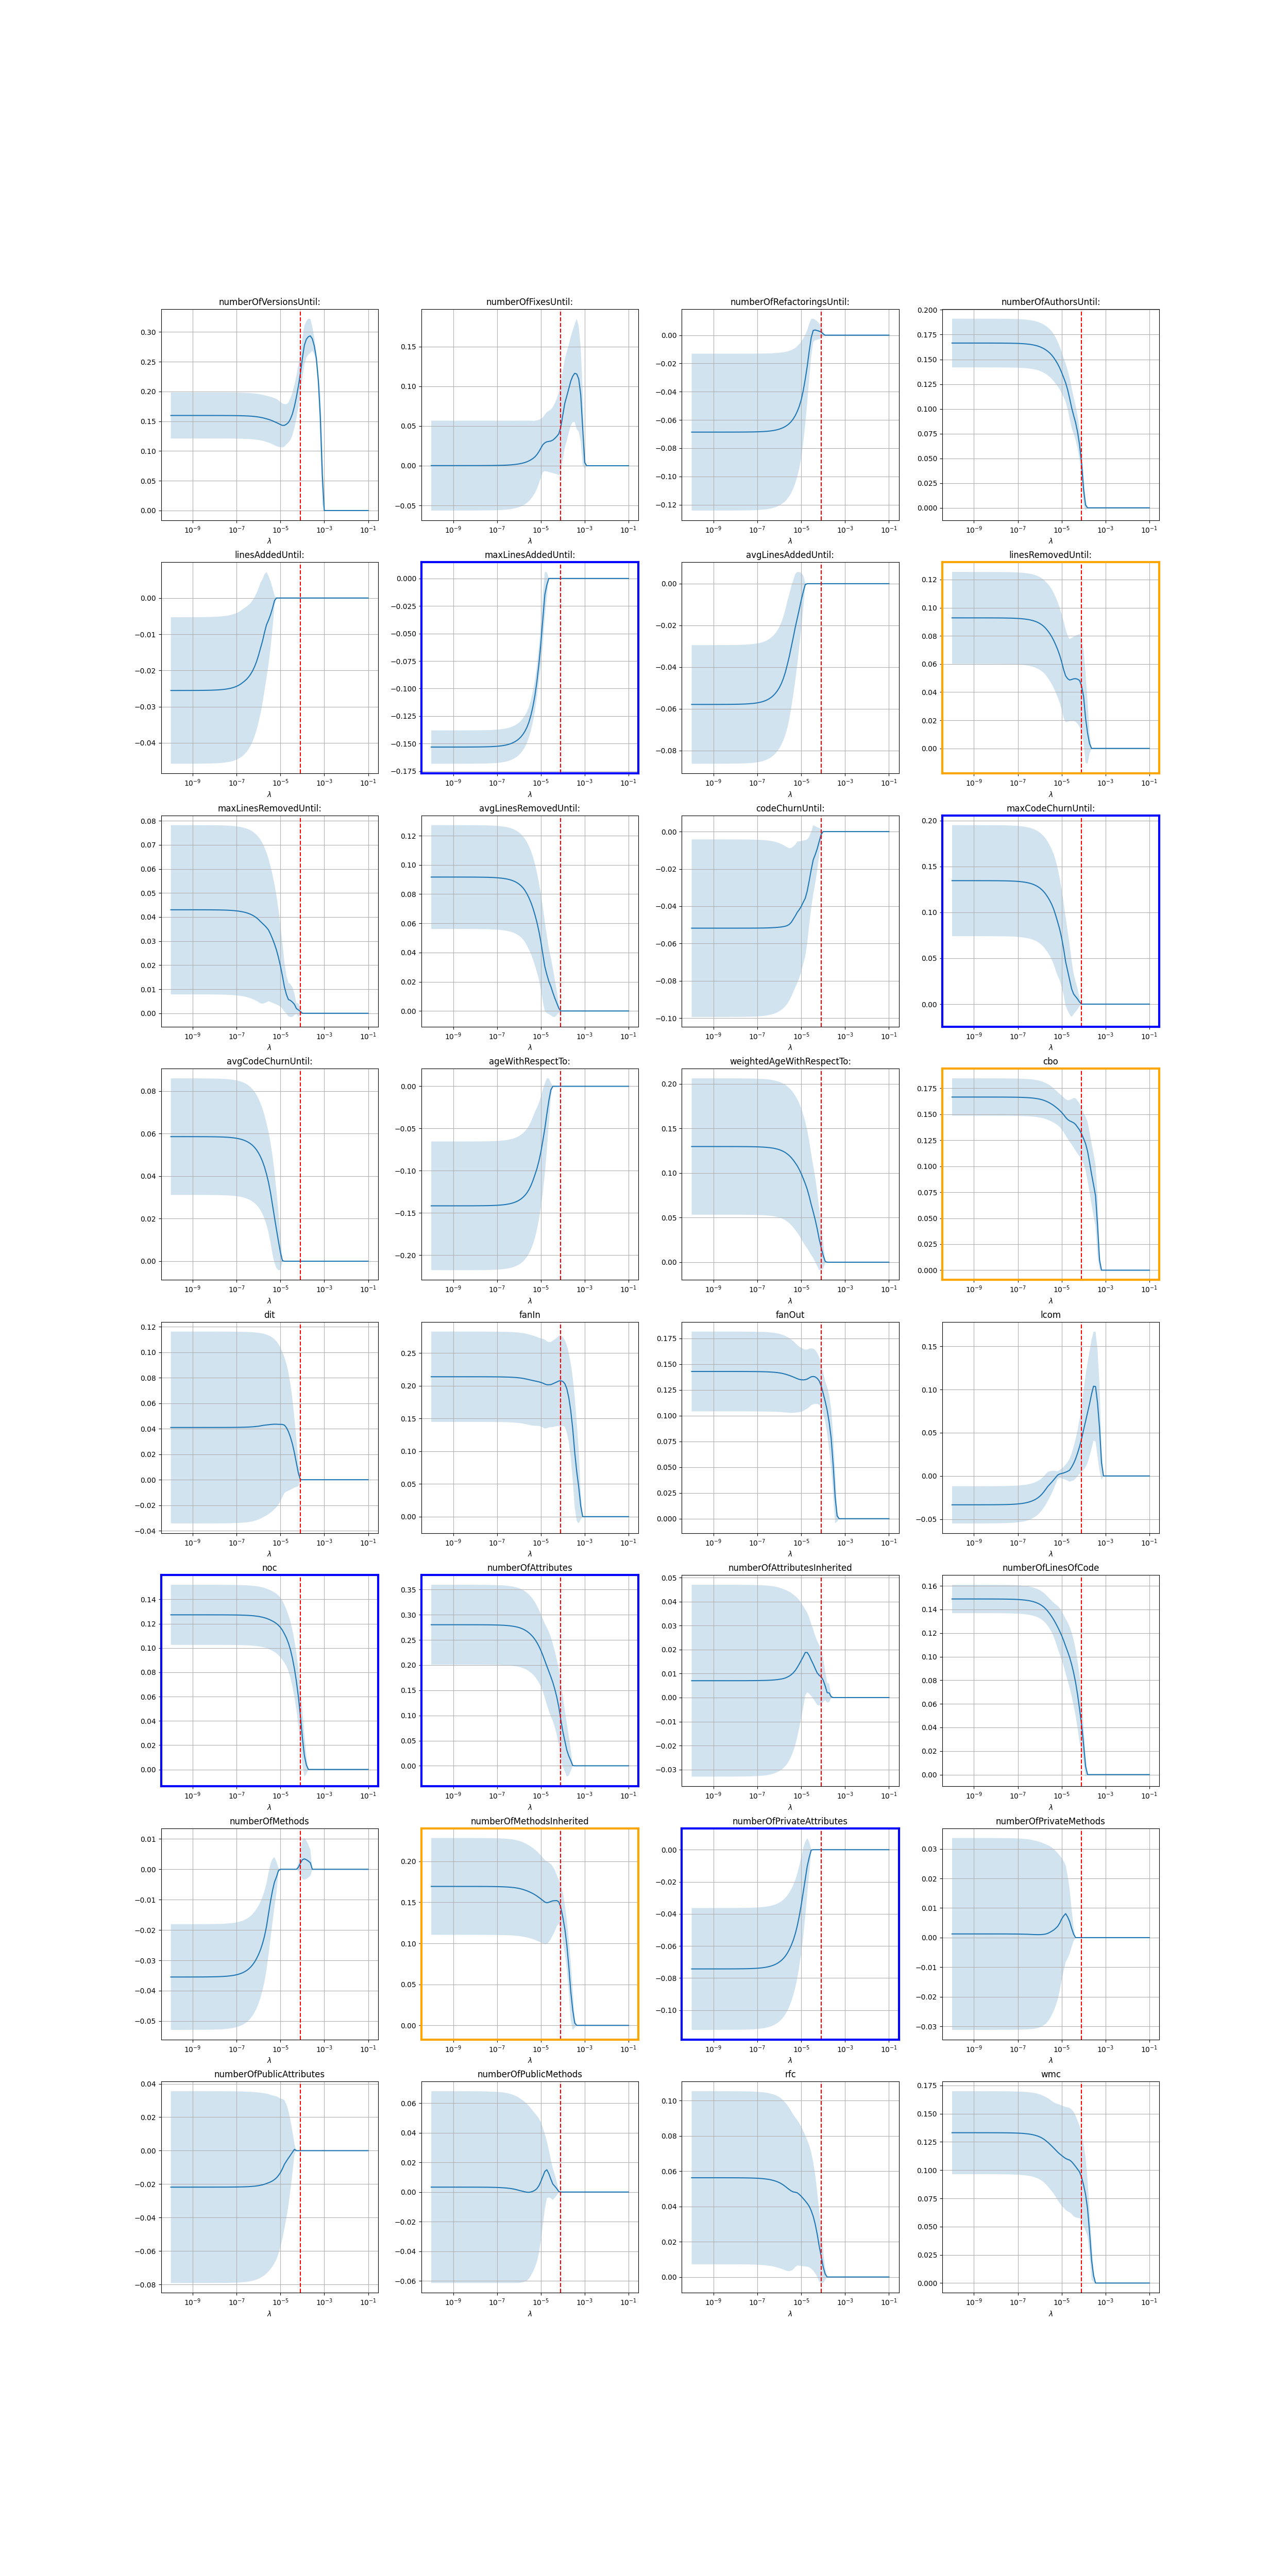
\includegraphics[width=0.5\linewidth]{extra_plots/poisson_regression_lasso_coefficients_log_transform.png}
    \caption{The coefficients of the \textbf{Poisson} regression model for all 32 features w.r.t. $\lambda$ when using the \textbf{log-transformed and normalized} data. The plots highlighted in \textbf{blue} are features found by the stepwise search model using AIC. We further highlighted in \textbf{orange} the features found by the stepwise search when using BIC. We advise the reader to view this report digitally to make the most of this plot.}
    \label{fig:coefficients_lambda_log_transformed_and_normalized}
\end{figure}

\begin{figure}[t]
    \centering
    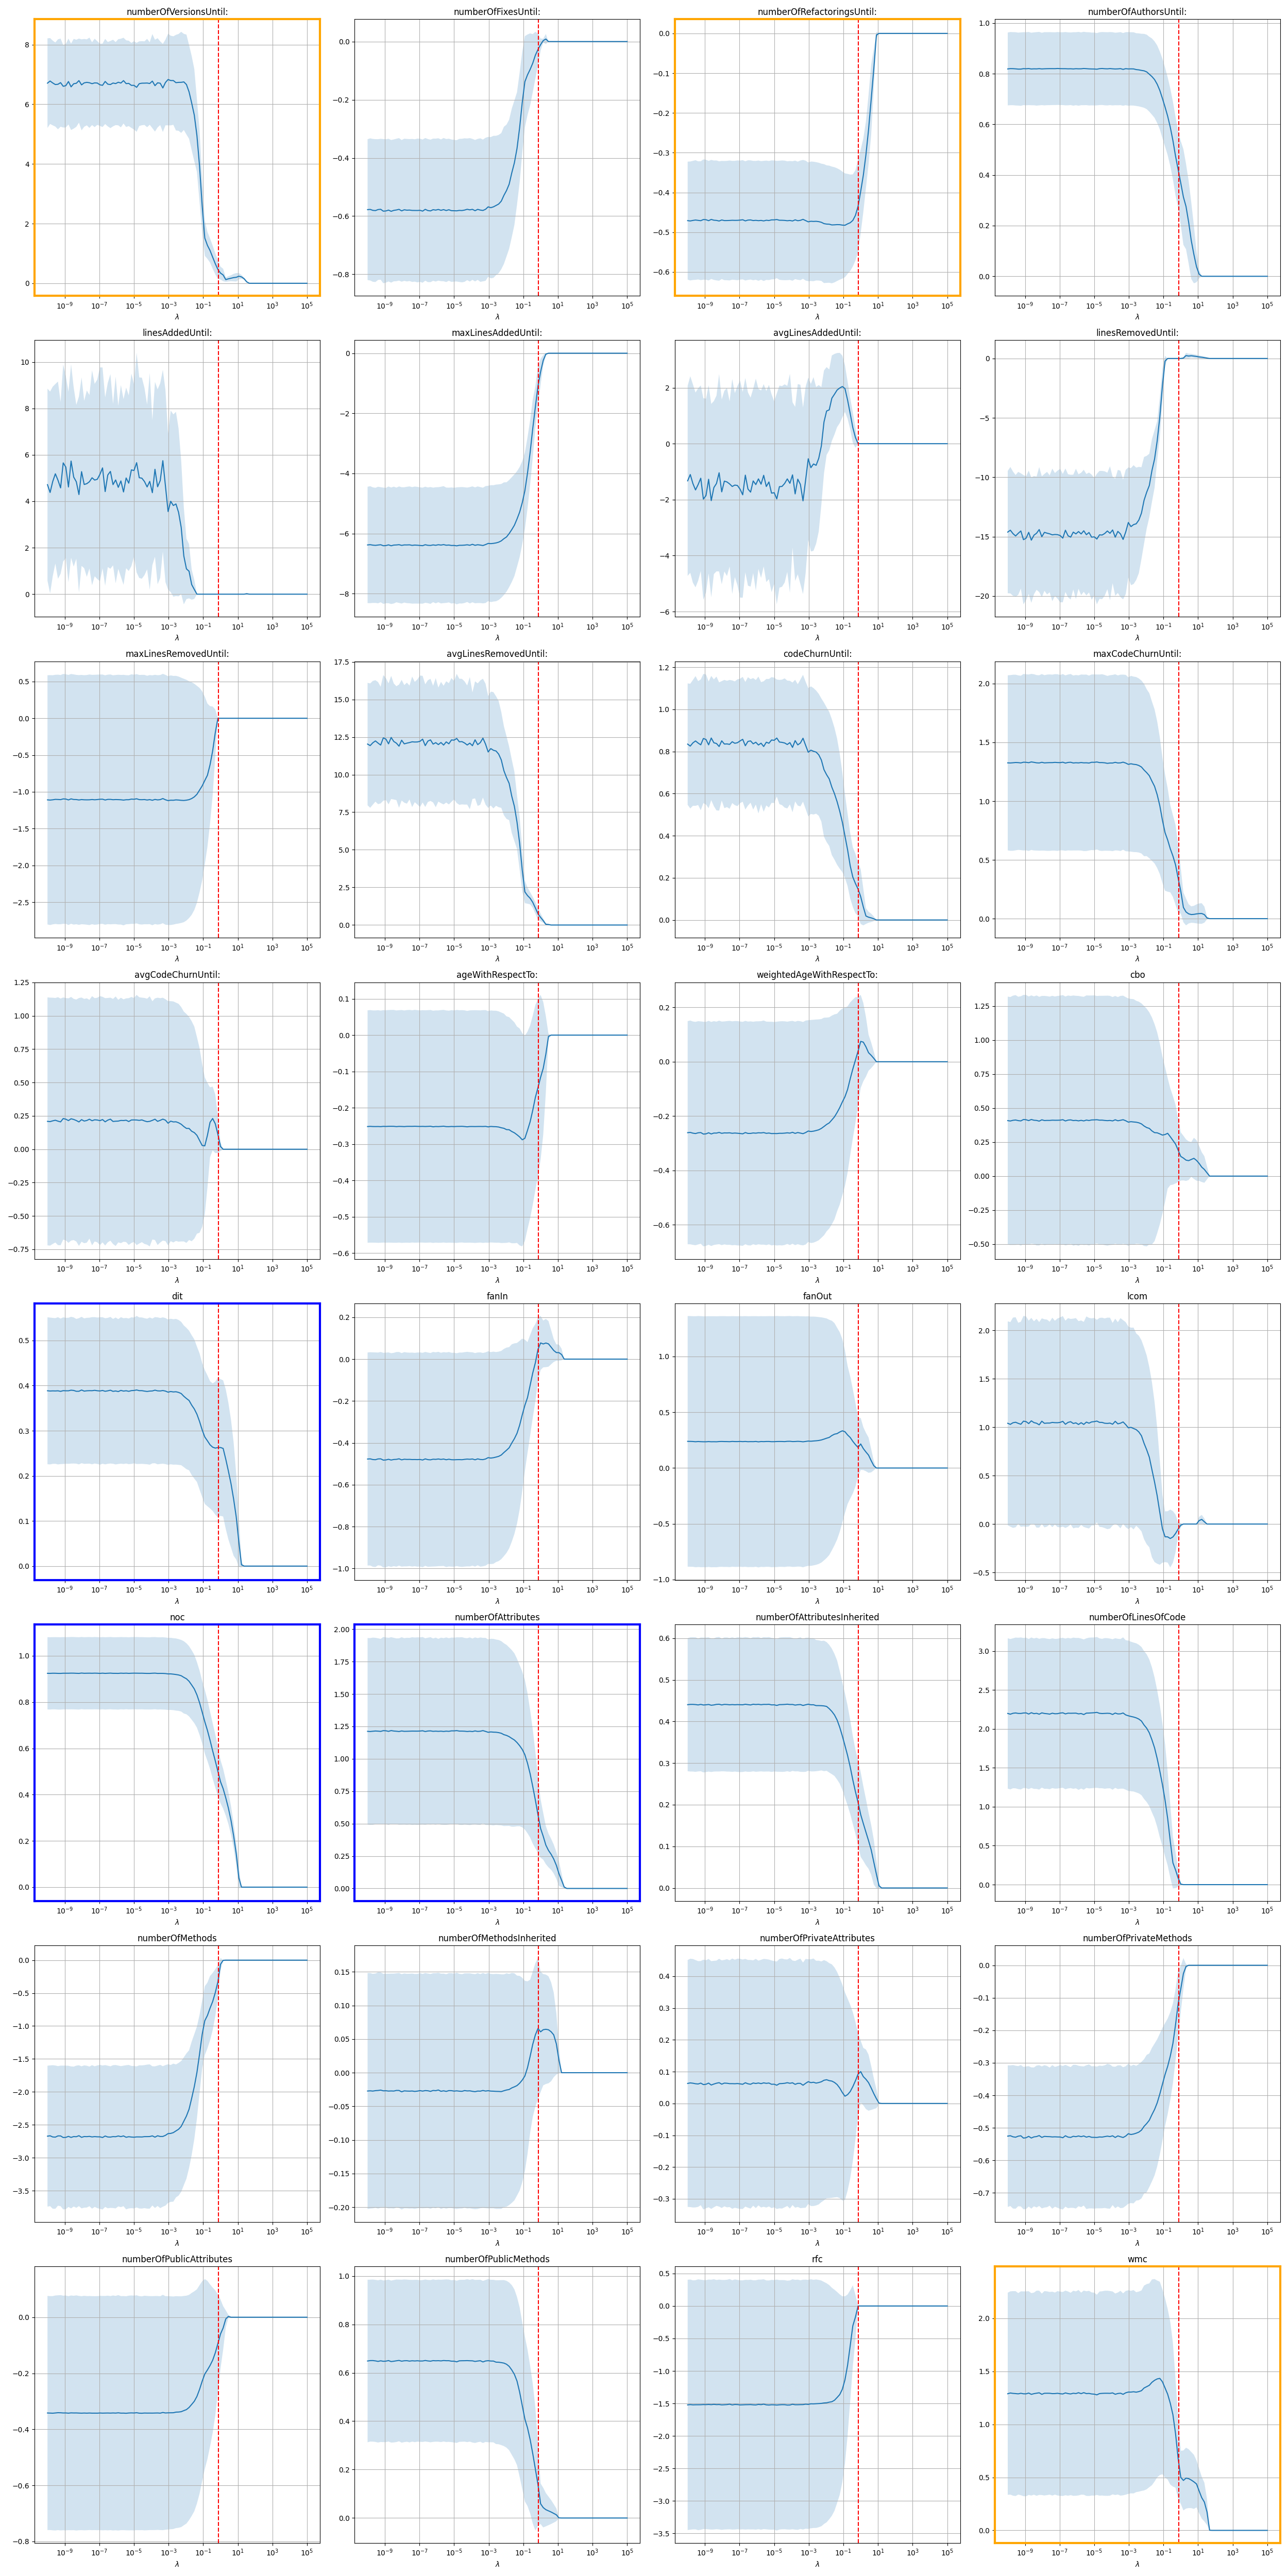
\includegraphics[width=0.5\linewidth]{extra_plots/logistic_regression_lasso_coefficients_log_transform.png}
    \caption{The coefficients of the \textbf{Logistic} regression model for all 32 features w.r.t. $\lambda$ when using the \textbf{log-transformed and normalized} data. The plots highlighted in \textbf{blue} are features found by the stepwise search model using AIC. We further highlighted in \textbf{orange} the features found by the stepwise search when using BIC. We advise the reader to view this report digitally to make the most of this plot.}
    \label{fig:logistic_regression_lasso_coefficients_log_transform}
\end{figure}

\begin{figure}[tp]
    \centering
    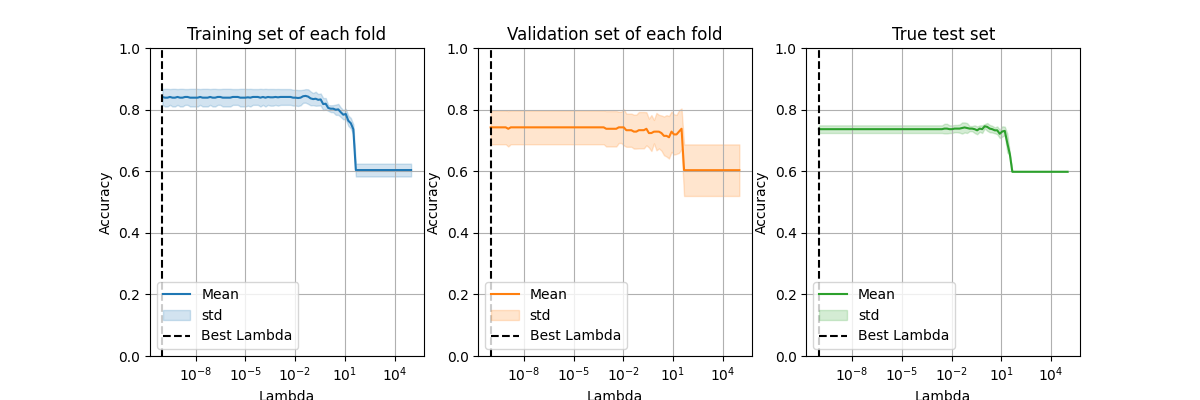
\includegraphics[width=\linewidth]{extra_plots/logistic_regression_lasso_deviance_vs_lambda_no_log_transform.png}
    \caption{Accuracy w.r.t. $\lambda$ for the $L_1$-lasso \textbf{logistic} regression for the just normalized data.}
    \label{fig:logistic_regression_lasso_deviance_vs_lambda_no_log_transform}
\end{figure}




\begin{table}[htbp]
    \centering
    \begin{tabular}{l c c}
        \toprule
        \textbf{Feature} & \textbf{Coefficient} & $\frac{\mathbb{E}[y\mid x+\delta_i]}{\mathbb{E}[y\mid x]}$ \\
        \midrule
        \texttt{noc} & $0.734$ & $3.335$ \\
        \texttt{dit} & $0.567$ & $3.219$ \\
        \texttt{cbo} & $3.020$ & $1.319$ \\
        \texttt{numberOfPublicMethods} & $1.631$ & $1.277$ \\
        \texttt{numberOfAuthorsUntil:} & $0.507$ & $1.269$ \\
        \texttt{numberOfPrivateMethods} & $0.654$ & $1.129$ \\
        \texttt{numberOfAttributes} & $0.932$ & $1.071$ \\
        \texttt{numberOfAttributesInherited} & $0.335$ & $1.059$ \\
        \texttt{wmc} & $2.731$ & $1.050$ \\
        \texttt{avgLinesRemovedUntil:} & $0.567$ & $1.044$ \\
        \texttt{numberOfPrivateAttributes} & $0.197$ & $1.039$ \\
        \texttt{numberOfMethodsInherited} & $0.333$ & $1.024$ \\
        \texttt{weightedAgeWithRespectTo:} & $0.384$ & $1.012$ \\
        \texttt{linesRemovedUntil:} & $3.676$ & $1.010$ \\
        \texttt{numberOfVersionsUntil:} & $0.175$ & $1.009$ \\
        \texttt{maxLinesAddedUntil:} & $1.290$ & $1.008$ \\
        \texttt{numberOfLinesOfCode} & $1.506$ & $1.007$ \\
        \texttt{lcom} & $0.988$ & $1.004$ \\
        \texttt{linesAddedUntil:} & $1.492$ & $1.003$ \\
        \texttt{maxCodeChurnUntil:} & $-0.261$ & $0.998$ \\
        \texttt{ageWithRespectTo:} & $-0.176$ & $0.998$ \\
        \texttt{codeChurnUntil:} & $-0.819$ & $0.997$ \\
        \texttt{avgLinesAddedUntil:} & $-0.197$ & $0.992$ \\
        \texttt{avgCodeChurnUntil:} & $-0.252$ & $0.988$ \\
        \texttt{maxLinesRemovedUntil:} & $-2.965$ & $0.977$ \\
        \texttt{rfc} & $-3.512$ & $0.966$ \\
        \texttt{numberOfPublicAttributes} & $-1.004$ & $0.916$ \\
        \texttt{fanOut} & $-1.009$ & $0.894$ \\
        \texttt{fanIn} & $-1.324$ & $0.763$ \\
        \texttt{numberOfMethods} & $-3.550$ & $0.727$ \\
        \texttt{numberOfFixesUntil:} & $-1.390$ & $0.670$ \\
        \texttt{numberOfRefactoringsUntil:} & $-0.542$ & $0.258$ \\
        \bottomrule
    \end{tabular}
    \caption{Coefficients of the best \textbf{Logistic} regression model found with \textbf{$L_1$-regularization} for the \textbf{just normalized} dataset.}
    \label{tab:features_coeff_logistic_normalized}
\end{table}
